\documentclass{article}

\usepackage{graphicx}
\usepackage{tikz}
\usepackage{tikzsymbols}
\usetikzlibrary{calc,patterns,shapes.geometric}
\pagestyle{empty}
\usepackage[margin=0pt]{geometry}
\geometry{papersize={14in,12in}}

\def\centerarc[#1](#2)(#3:#4:#5){\draw[#1] ($(#2)+({#5*cos(#3)},{#5*sin(#3)})$) arc (#3:#4:#5);}

\begin{document}
	\begin{figure}
		\centering
		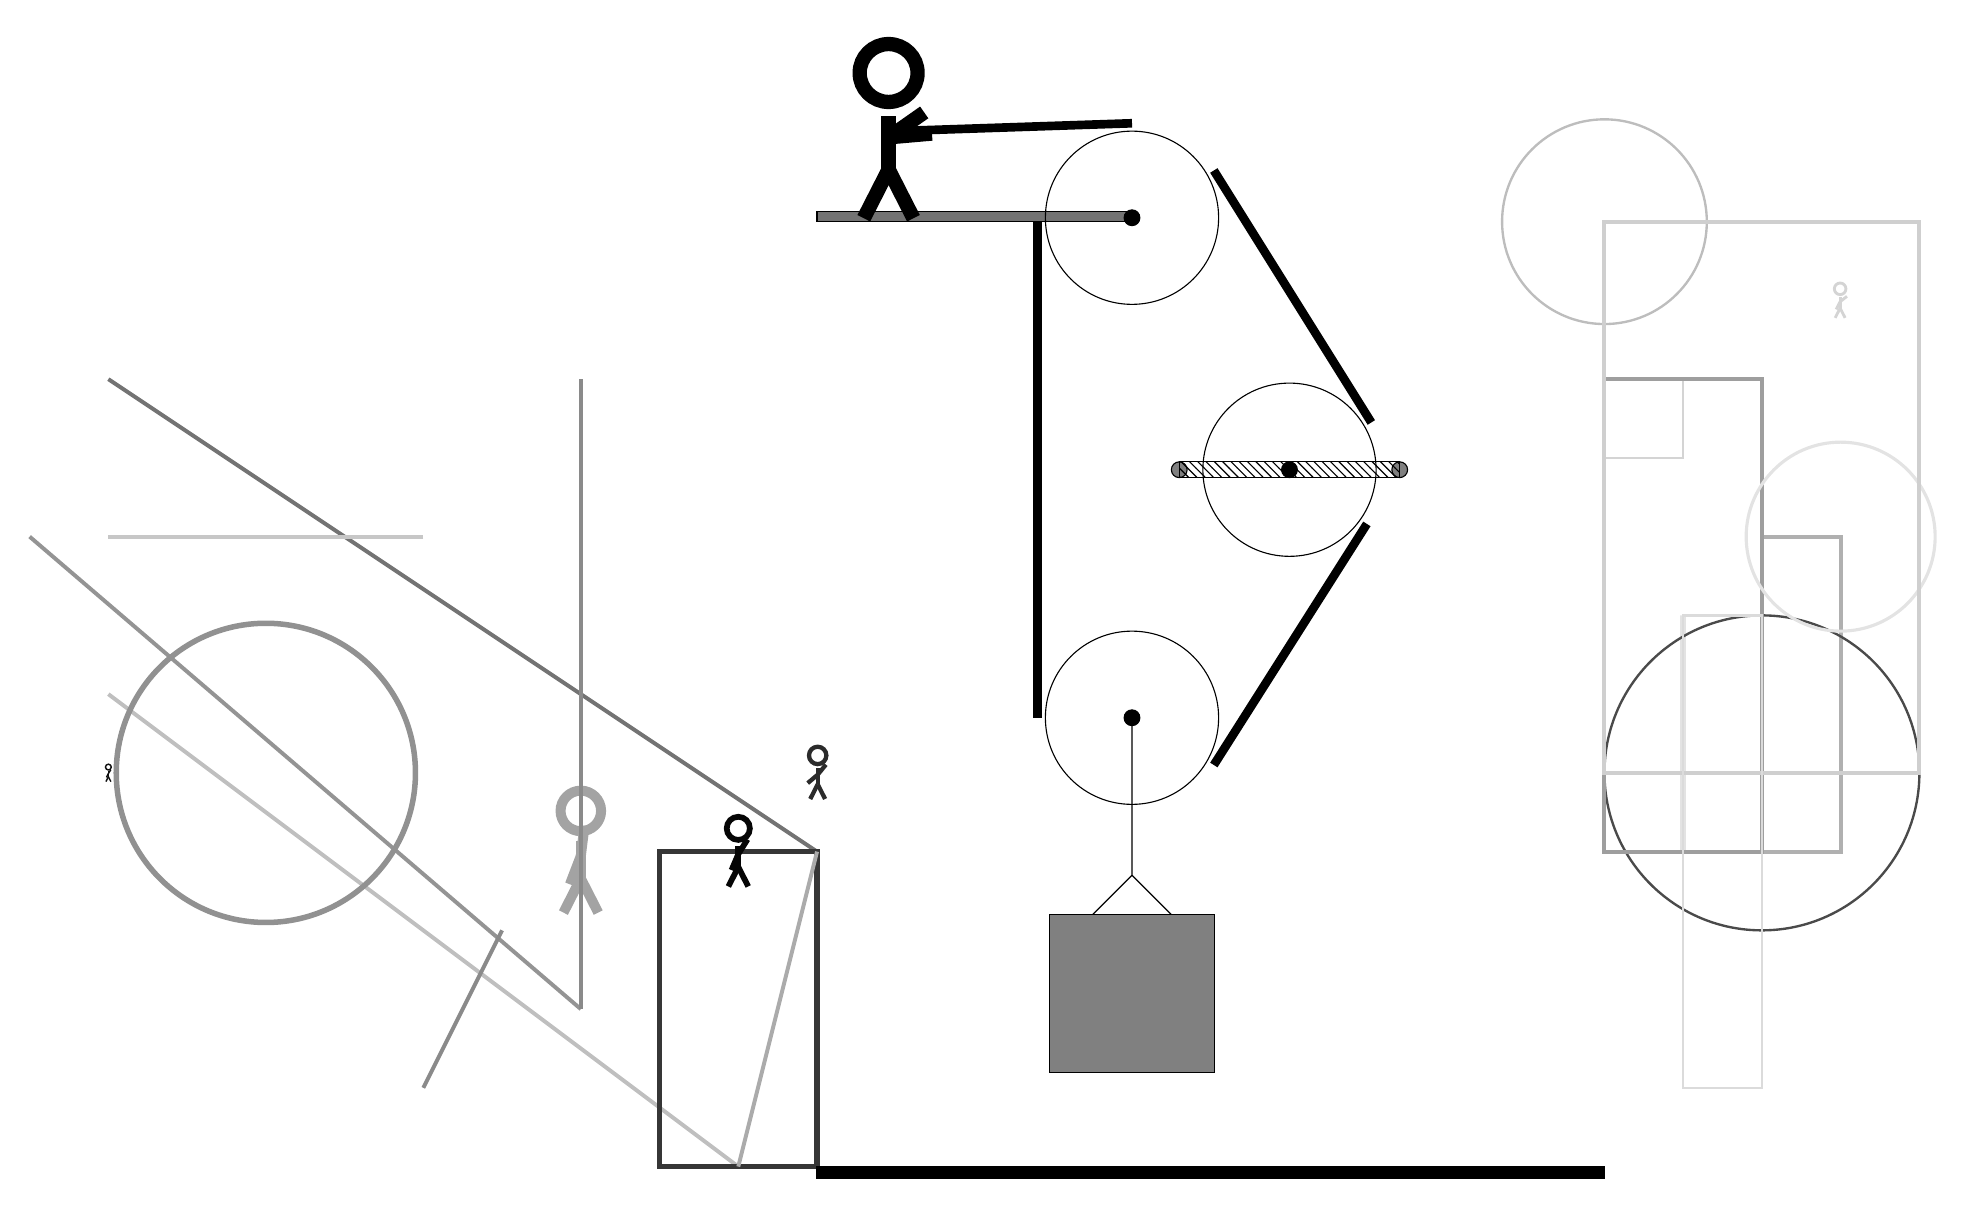
\begin{tikzpicture}
			%%%%% START %%%%%
			
			\draw[fill=black!55] (-2, 9) rectangle (2, 9.125);
			
			\draw (2, 2.7) circle (1.1);
			\draw[fill=black] (2, 2.7) circle (0.1);
			
			\draw (2, 9.05) circle (1.1);
			\draw[fill=black] (2, 9.05) circle (0.1);
			
			\draw[fill=white](4, 5.85) circle (1.1);
			\draw[fill=black] (4, 5.85) circle (0.1);
			\draw[fill=black!50] (2.6, 5.85) circle (0.1);
			\draw[fill=black!50] (5.4, 5.85) circle (0.1);
			\draw[pattern=north west lines, pattern color=black] (2.6, 5.95) rectangle (5.4, 5.75);
			
			\draw (2, 2.7) -- (2, 0.7) -- (1.5, 0.2) -- (2.5, 0.2) -- (2, 0.7);
			\draw[fill=black!50] (0.95, 0.2) rectangle (3.05, -1.8);
			
			\draw[line width=1.1mm] (0.8, 9) -- (0.8, 2.7);
			\centerarc[line width=1.1mm](2, 2.7)(180:330:1.2000000000000002);
			\draw[line width=1.1mm](3.0392, 2.1) -- (4.983, 5.1617);
			\centerarc[line width=1.1mm](4, 5.85)(390:325:1.2000000000000002);
			\draw[line width=1.1mm](5.0392, 6.45) -- (3.0392, 9.65);
			\centerarc[line width=1.1mm](2, 9.05)(30:90:1.2000000000000002);
			\draw[line width=1.1mm](2, 10.25) -- (-1, 10.15);
			
			\node at (-1, 10.15) {\Strichmaxerl[10][-175][35]};
			
			\draw[line width=0.5mm, color=black!25](-3, -3) -- (-11, 3);
			
			\draw[line width=0.5mm, color=black!42](-5, -1) -- (-12, 5);
			\node[line width=0.5mm, color=black!17] at (11, 8) {\Strichmaxerl[2][63][38]};
			\draw[line width=0.5mm, color=black!55](-2, 1) -- (-11, 7);
			
			\node[line width=0.5mm, color=black!36] at (-5, 1) {\Strichmaxerl[7][69][83]};
			\draw[line width=0.2mm, color=black!17] (9, 7) rectangle (8, 6);
			\draw [line width=0.3mm, color=black!26](8, 9) circle (1.3);
			\node[line width=0.2mm, color=black!94] at (-11, 2) {\Strichmaxerl[1][63][57]};
			\draw[line width=0.5mm, color=black!46](-6, 0) -- (-7, -2);
			\draw[line width=0.5mm, color=black!22](-7, 5) -- (-11, 5);
			\draw[line width=0.7mm, color=black!11] (9, 1) rectangle (9, 4);
			\draw[line width=0.5mm, color=black!31] (10, 5) rectangle (11, 1);
			\draw [line width=0.6mm, color=black!70](11, 4) circle (0.0);
			\node[line width=0.4mm, color=black!83] at (-2, 2) {\Strichmaxerl[3][40][51]};
			\draw[line width=0.5mm, color=black!46](-5, -1) -- (-5, 7);
			\draw [line width=0.3mm, color=black!71](10, 2) circle (2.0);
			
			\draw[line width=0.5mm, color=black!38] (8, 7) rectangle (10, 1);
			\draw[line width=0.7mm, color=black!79] (-2, -3) rectangle (-4, 1);
			\draw [line width=0.4mm, color=black!11](11, 5) circle (1.2);
			\draw[line width=0.5mm, color=black!19] (8, 9) rectangle (12, 2);
			\node[line width=0.6mm, color=black!98] at (-3, 1) {\Strichmaxerl[4][67][58]};
			\draw[line width=0.5mm, color=black!33](-3, -3) -- (-2, 1);
			
			\draw [line width=0.7mm, color=black!43](-9, 2) circle (1.9);
			\draw[line width=0.3mm, color=black!14] (10, -2) rectangle (9, 4);
			
			\draw[fill=black] (-2, -3) rectangle (8, -3.15);
			
			%%%%% END %%%%%
		\end{tikzpicture}
	\end{figure}	
\end{document}